% !TEX encoding = UTF-8
% !TEX TS-program = pdflatex
% !TEX root = ../tesi.tex

%**************************************************************
\chapter{Blockchain}
\label{cap:blockchain}

\section{Struttura e funzionamento}

La \gls{blockchaing} è un una tecnologia che si basa su un \textit{database} distribuito che viene acceduto contemporaneamente da più nodi di una rete \textit{peer-to-peer}, ossia una rete di macchine paritetiche che comunicano tra di loro direttamente, senza bisogno di passare attraverso dei nodi aventi delle funzioni di gestione della rete e del traffico presente al suo interno.\\
Attraverso questa rete, i nodi possono effettuare delle transazioni senza il bisogno di un entità terza che faccia da garante intermediario, sfruttando le proprietà della crittografia. Infatti, tramite il suo impiego, le tecnologie \gls{blockchaing} permettono di garantire l'affidabilità sulla veridicità e autenticità delle operazioni e delle comunicazioni effettuate tra individui che non hanno fiducia l'uno dell'altro.
\begin{figure}[H] 
	\centering 
	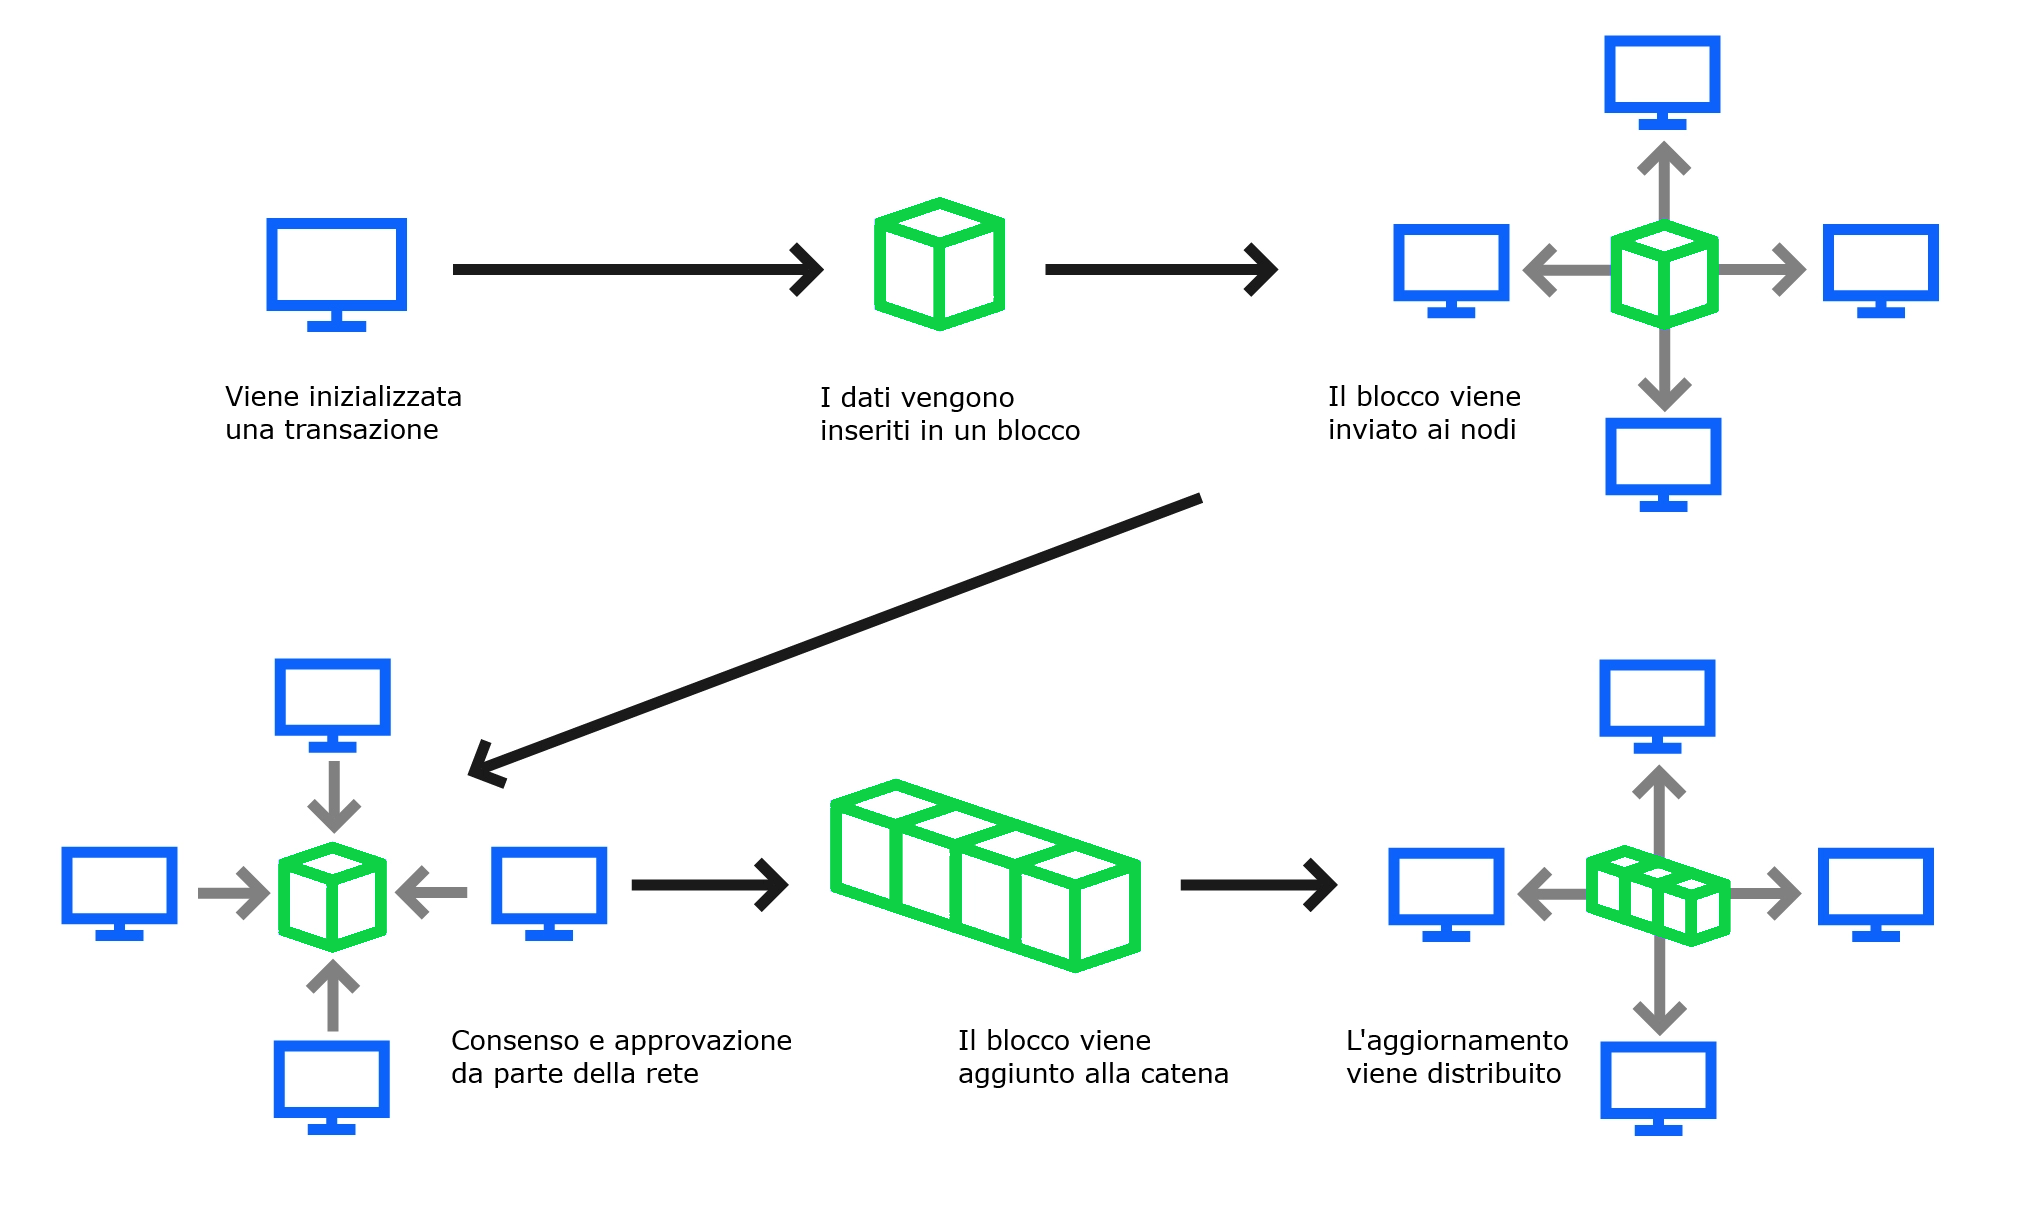
\includegraphics[width=\textwidth]{blockchain} 
	\caption{Esecuzione di una transazione tramite la \gls{blockchaing}}
\end{figure}
\newpage
\noindent
In questo contesto, per transazione tra due utenti di una \gls{blockchaing} si intende qualsiasi trasmissione di informazioni, le quali dovranno essere memorizzate all'interno del \textit{database} distribuito, in modo da essere accessibili da parte di tutti i nodi della rete. A questo scopo, le informazioni da trasferire vengono incluse in delle strutture dati chiamate blocchi; questi contengono al loro interno più transazioni e, affinché possano essere aggiunti alla \gls{blockchaing}, ne deve essere verificata la validità e l'affidabilità da parte di tutti i nodi della rete. Per compiere quest'operazione vengono utilizzati opportuni algoritmi di consenso distribuito il cui compito è il raggiungimento di un accordo condiviso su quali blocchi debbano essere aggiunti e quali invece scartati. Una volta che un blocco viene verificato ogni partecipante alla \gls{blockchaing} aggiorna la sua copia locale del \textit{database} con le nuove informazioni.\\
Una \gls{blockchaing} può essere vista come l'insieme di tre parti distinte:

\begin{itemize}
	\item \textbf{\textit{software}:} il \textit{database} distribuito, accessibile solamente in lettura e in inserimento, in cui le informazioni contenute sono verificate come affidabili tramite un protocollo per il consenso distribuito, il quale permette a tutti i nodi di essere d'accordo sull'inserimento o meno di nuove informazioni e, una volta raggiunta l'intesa su un certo dato, gli conferisce lo \textit{status} di valido e non più modificabile; fa parte del \textit{software} anche il livello di rete che realizza lo scambio di informazioni tra i diversi nodi appartenenti alla \gls{blockchaing}
	\item \textbf{crittografia:} impiegata per firmare digitalmente e verificare l'autenticità e l'integrità di tutte le transazioni e i processi di scambio dati tra i nodi della rete;
	\item \textbf{criptovaluta:} una risorsa digitale nativa della \gls{blockchaing}, alla quale viene associato un controvalore in moneta a corso legale, che fornisce gli incentivi economici per l'utilizzo e il mantenimento della rete da parte dei nodi, in modo tale che risulti più conveniente agire in modo onesto piuttosto che in modo disonesto.
\end{itemize}
Attraverso la \gls{blockchaing} è possibile aumentare la trasparenza e la tracciabilità delle filiere produttive e facilitare l'accesso alle transazioni tra privati, aumentandone l'efficienza; il tutto senza bisogno di intermediari che richiedano il pagamento di commissioni e il mantenimento di informazioni personali.

\section{Consenso}

Il protocollo di consenso è un meccanismo resistente agli errori che viene utilizzato all'interno della \gls{blockchaing} per raggiungere l'accordo su un singolo stato della rete tra tutti i nodi distribuiti che la compongono. Questo protocollo è fondamentale per il funzionamento della rete in quanto, dato che ogni nodo può inviare delle nuove transazioni da aggiungere alla \gls{blockchaing}, è necessario che tutte siano sempre controllate e verificate, in modo da raggiungere il consenso su quali debbano essere aggiunte e quali invece rifiutate.\\
Esistono diversi meccanismi di consenso che differiscono per il modo in cui riescono a garantire la fiducia tra i diversi nodi della rete, al fine di raggiungere l'accordo sulle operazioni da eseguire. I principali sono:

\begin{itemize}
	\item \textbf{\gls{pow}:} è stato il primo protocollo di consenso utilizzato ad è conosciuto con il nome di \textit{mining}, per cui i nodi vengono chiamati minatori; questi devono risolvere problemi matematici molto complessi dal punto di vista computazionale, senza però alcun fine pratico, per poter creare un blocco, validare le transazioni in esso contenute e quindi ricevere una ricompensa, in termini di un certo ammontare di criptovaluta, per il lavoro svolto;
	\item \textbf{\gls{pos}:} è un protocollo ideato per essere utilizzato nei contesti in cui i nodi di una rete hanno un proprio interesse nel contribuire al funzionamento della \gls{blockchaing}; in questo scenario viene creato un sottoinsieme di nodi che ha la possibilità di validare i nuovi blocchi e il singolo nodo che avrà il compito di inserire il blocco attuale viene scelto in casualmente tra tutti; per garantire l'affidabilità dei nodi validatori questi sono obbligati a mantenere in stato di fermo un certo ammontare di criptovaluta, in modo da dare prova della loro volontà di agire negli interessi della rete e non nei propri.
\end{itemize}

\section{Immutabilità}

All'interno di una \gls{blockchaing}, ogni volta che una nuova transazione viene inserita, col consenso di tutti i nodi partecipanti alla rete, questa diventa immutabile e non può più essere modificata o eliminata. Infatti, ogni blocco di transazioni all'interno della \gls{blockchaing} sfrutta una funzione crittografica chiamata \textit{hash}, la quale genera una stringa alfanumerica che rappresenta l'intero contenuto del blocco; questa, per le proprietà con cui viene costruita, varia di molto anche per minime modifiche dell'\textit{input} che l'ha generata.\\
Ogni blocco, quindi, contiene al suo interno il proprio valore \textit{hash} e quello del blocco precedente: il primo funge da firma digitale e garantisce l'integrità dei dati su cui è stato calcolato, il secondo invece è necessario all'identificazione del blocco precedente, per poter ripercorrere la \gls{blockchaing} fino all'origine. Sfruttando queste due informazioni si può garantire l'immutabilità in quanto, se venisse fatta una modifica ad un blocco, il suo \textit{hash} verrebbe a sua volta modificato e quindi differirebbe da quello memorizzato all'interno del suo successore, invalidando la catena.

\section{Finalità}

Con finalità si intende il fatto che un blocco validato non può più essere revocato dalla \gls{blockchaing}; in base al protocollo di consenso utilizzato, può essere raggiunta con modalità e in tempi differenti. I principali tipi di finalità sono:

\begin{itemize}
	\item \textbf{finalità probabilistica:} questa tipologia di finalità è caratteristica dei protocolli di tipo \textit{chain-based}, i quali solitamente utilizzando il \gls{pow} come meccanismo di consenso; in queste \gls{blockchaing} la probabilità che un blocco non sia revocato aumenta all'aumentare del numero di blocchi ad esso successivi, quindi più profondo è un blocco più è alta la probabilità che faccia parte della diramazione più lunga della catena, cioè quella valida;
	\item \textbf{finalità istantanea:} questa tipologia di finalità è tipica dei protocolli di tipo \textit{PBFT-based}, i quali solitamente utilizzano il \gls{pos} come meccanismo di consenso; in queste \gls{blockchaing} un blocco è considerato finalizzato non appena viene aggiunto alla catena, in quanto, prima di poter procedere con l'aggiunta, il nuovo blocco deve essere prima proposto da un nodo e poi approvato tramite votazione dalla maggioranza o più dei nodi validatori presenti.
\end{itemize}
